% !TEX root=/home/tavant/these/manuscript/src/manuscript.tex

% \FloatBarrier
\section{Sheath model with polytropic electrons and electron emission}
\label{sec-fluid_poly_see}

\let\oldrightmark=\rightmark
\renewcommand\rightmark{\expandafter\MakeUppercase{Sheath with polytropic electron and SEE}}


\subsection{Definition of the sheath equation} \label{subsec-def_sheat_see}

We have seen in \cref{sec-PIC_poly} that even in the presence of electron emission from the wall, the electrons can be described using a polytropic state law.
The value of the polytropic index obtained from the mean electron density and temperature is for $\crover \geq 40 \,\volt$ is $\gamma = 1.36$.
% Using the electron distribution function, the evolution of the forward electron seems to follow a polytropic low of index $\gamma=1.28$.
Hence, we modify the polytropic sheath model of \cref{sec-fluid} to take into account the electron emission from the wall.
This modifies the current equality at the wall to
\begin{equation} \label{eq-see-J_eq}
  \Gamma_i = (1 - \rate) \Gamma_e.
\end{equation}

\paragraph{Sheath model with constant emission rate\\}

Using \cref{eq-gi,eq-ge,eq-tew} for $\Gamma_i$ and $\Gamma_e$, we obtain the equality
\begin{equation}\label{eq-sheathsee}
  (1 - \rate )\left[ 1 +\frac{\gamma -1}{\gamma} \frac{ \dphi_0}{ \Te_0}  \right]^{\frac{1}{\gamma - 1}} \sqrt{1 - \frac{\gamma -1}{\gamma}\frac{\dphi_0}{\Te_0}} = \sqrt{\frac{4 \gamma \pi m_e}{m_i}}
\end{equation}

Similarly to the case without electron emission in \cref{sec-fluid}, \cref{eq-sheathsee} cannot be solved analytically, but it can be solved numerically.
The solution for $\rate=0.8$ is compared to the case without electron emission ($\rate=0$) for a \ac{Xe} plasma in \cref{fig-dphi_see}.
As expected, the potential difference decreases with increasing $\rate$.
We see that the gap between the two cases decreases when $\gamma$ increases from 1 to 2.

\begin{figure}[!hbt]
  \centering
  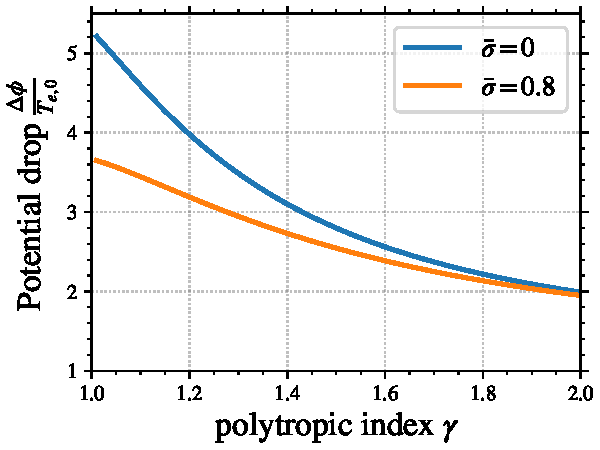
\includegraphics[width=\defaultwidth]{Sheath_drop_with_SEE.pdf}
  \caption{Potential drop $\dphi$ normalized by the bulk electron temperature $\Te_0$ as a function of the polytropic index $\gamma$ for a xenon plasma ($m_i = 131\,\atomicmass$). The emission rate $\rate$ is fixed either at $\rate=0$ or $\rate=0.8$.}
  \label{fig-dphi_see}
\end{figure}

\paragraph{Sheath model with varying emission rate\\}

In fact the electron emission rate is a function of the electron temperature at the wall.
Using the same hypothesis as in \cref{eq-ge} (mostly a Maxwellian \ac{EVDF} at the wall), we define the emission rate from \cref{eq-seemaxw} by
\begin{equation} \label{eq-seemaxw_poly}
  \rate = 
  \begin{cases}
    \ratemaxw(\Tew) =  \sigo + ( 1 - \sigo) \frac{ 2 \Tew  }{\crover} \\
    \ratecr \text{ \quad, if } \ratemaxw(\Tew) > \ratecr
  \end{cases}
\end{equation}
with $\ratecr = 0.983$ corresponding to the \ac{SCL} regime, and the electron temperature at the wall
\begin{equation} \label{eq-Tewall}
  \Tew = \Teb - \frac{\gamma - 1}{\gamma } \dphi.
\end{equation}


Noting $\chi = \frac{\gamma -1}{\gamma} \frac{ \dphi_0}{ \Teb} $, we finely obtain the sheath equation to be solved
\begin{equation} \label{eq-costseepoly}
  f(\chi) = \left[ 1 + \chi  \right]^{\frac{1}{\gamma - 1}} \sqrt{1 - \chi} - \frac{  \sqrt{4 \gamma m_e / m_i}}{1 - \rate (\Teb, \chi )} = 0.
\end{equation}

\Cref{eq-costseepoly} depends now explicitly on $\Teb$ though $\rate$.
Hence, the solution of $f(\chi)=0$ is no longer independent of $\Teb$, which adds a free parameter when solving the sheath equation.
\Cref{fig-costfunction} shows the evolution of $f(\chi)$ of \cref{eq-costseepoly} for $\gamma = 1.36$, $\Teb=40\,\volt$ and $\crover=50\,\volt$.

\begin{figure}[!hbt]
  \centering
  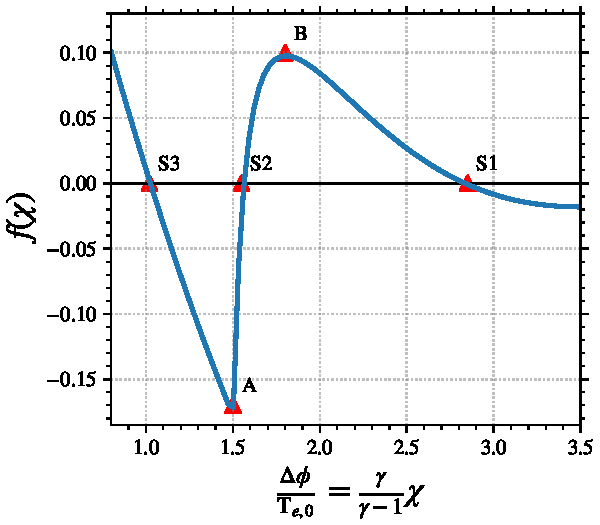
\includegraphics[width=\defaultwidth]{cost_function_solo}
  \caption{Value of $f(\chi)$ of \cref{eq-costseepoly} for $\gamma = 1.36$, $\Teb=40\,\volt$ and $\crover=50\,\volt$. The five red triangular markers represents five points of interest\string: the three markers S1, S2, and S3 are solutions of $f(\chi) = 0$; and the markers A and B are two local extrema. }
  \label{fig-costfunction}
\end{figure}

We see that $f(\chi)$ of \cref{eq-costseepoly} is rather complex.
Five points of interest are marked and labeled in \cref{fig-costfunction} to ease the reading\string: 
\begin{enumerate}
  \item S1, S2, and S3 represents the points at which $f(\chi)=0$, i.e. the solutions of  \cref{eq-costseepoly}
  \item A and B are two local extrema.
\end{enumerate}

The courbe $f(\chi)$ is composed of two continuous branches that join at the point A in \cref{fig-costfunction}.
The two branches corresponds to the two cases of \cref{eq-seemaxw_poly}. Hence, the point A corresponds to the value of $\dphi/\Teb$ for which  \[ \sigo + ( 1 - \sigo) \frac{ 2 \Tew  }{\crover} = \ratecr = 0.983. \]

The branch at the left of A corresponds to the \ac{SCL} regime, and has one solution S3 to $f(\chi)=0$ at $\dphi / \Teb \simeq 1$.
This solutions is the same as in the isothermal case \citep{hobbs1967}.
The branch at the right of A passes by a local maximum B and presents two roots S1 and S3.

The existence of the three solutions depends on the values of $\crover$, $\Teb$ and $\gamma$.
\Cref{fig-costfunction_multiple} shows the impact of the evolution of $\Teb$ and $\crover$, with $\gamma$ constant.
We can see that when $\Teb$ decreases, or $\crover$ increases, the points A and B move upward.
Consequently, for low values of $\Teb$ (respectively large values of $\crover$) the point A can be above the line $f(\chi) = 0$, hence  \cref{eq-costseepoly} presents only the root S1.
In contrast for high values of $\Teb$ (respectively low values of $\crover$) the point B is below $f(\chi) = 0$, so that only S3 is solution of  \cref{eq-costseepoly}.
For intermediate values of $\Teb$ and $\crover$, A and B are located on both sides of $f(\chi) = 0$, so that the three roots S1, S2, and S3 exist.
\renewcommand\subfigurewidth{0.47\textwidth}

\begin{figure}[!hbt]
  \centering
  \begin{tabular}{@{} c c}
    \subfigure{cost_function_bis.pdf}{a}{25,25} &
    \subfigure{cost_function_2bis.pdf}{b}{25,25} \\
  \end{tabular}
  \caption{Value of $f(\chi)$ of \cref{eq-costseepoly} for $\gamma = 1.36$ and different values of $\Teb$ and $\crover$. ({\bf a}) shows the impact of the evolution of $\Teb$ with $\crover=50\,\volt$, and ({\bf b}) shows the impact of the evolution of $\crover$ with $\Teb=35\,\volt$. }
  \label{fig-costfunction_multiple}
\end{figure}

\Cref{fig-schematic-solutions} illustrates the three coexisting sheath solutions.
The red solid line  with the largest potential drop to the wall represents the solution S1, which is the standard sheath.
This solutions leads to the largest electron temperature drop to the wall, hence the smallest \ac{SEE} rate.
The dashed blue line, with a potential well close to the wall, corresponds to the root S3 in the \acs{SCL} regime, for which $\rate=\ratecr$ and with $\dphi \simeq \Teb$.
Lastly, the dash-dotted green line represents S2 the intermediate solution.
 
\begin{figure}[hbtp]
  \centering
  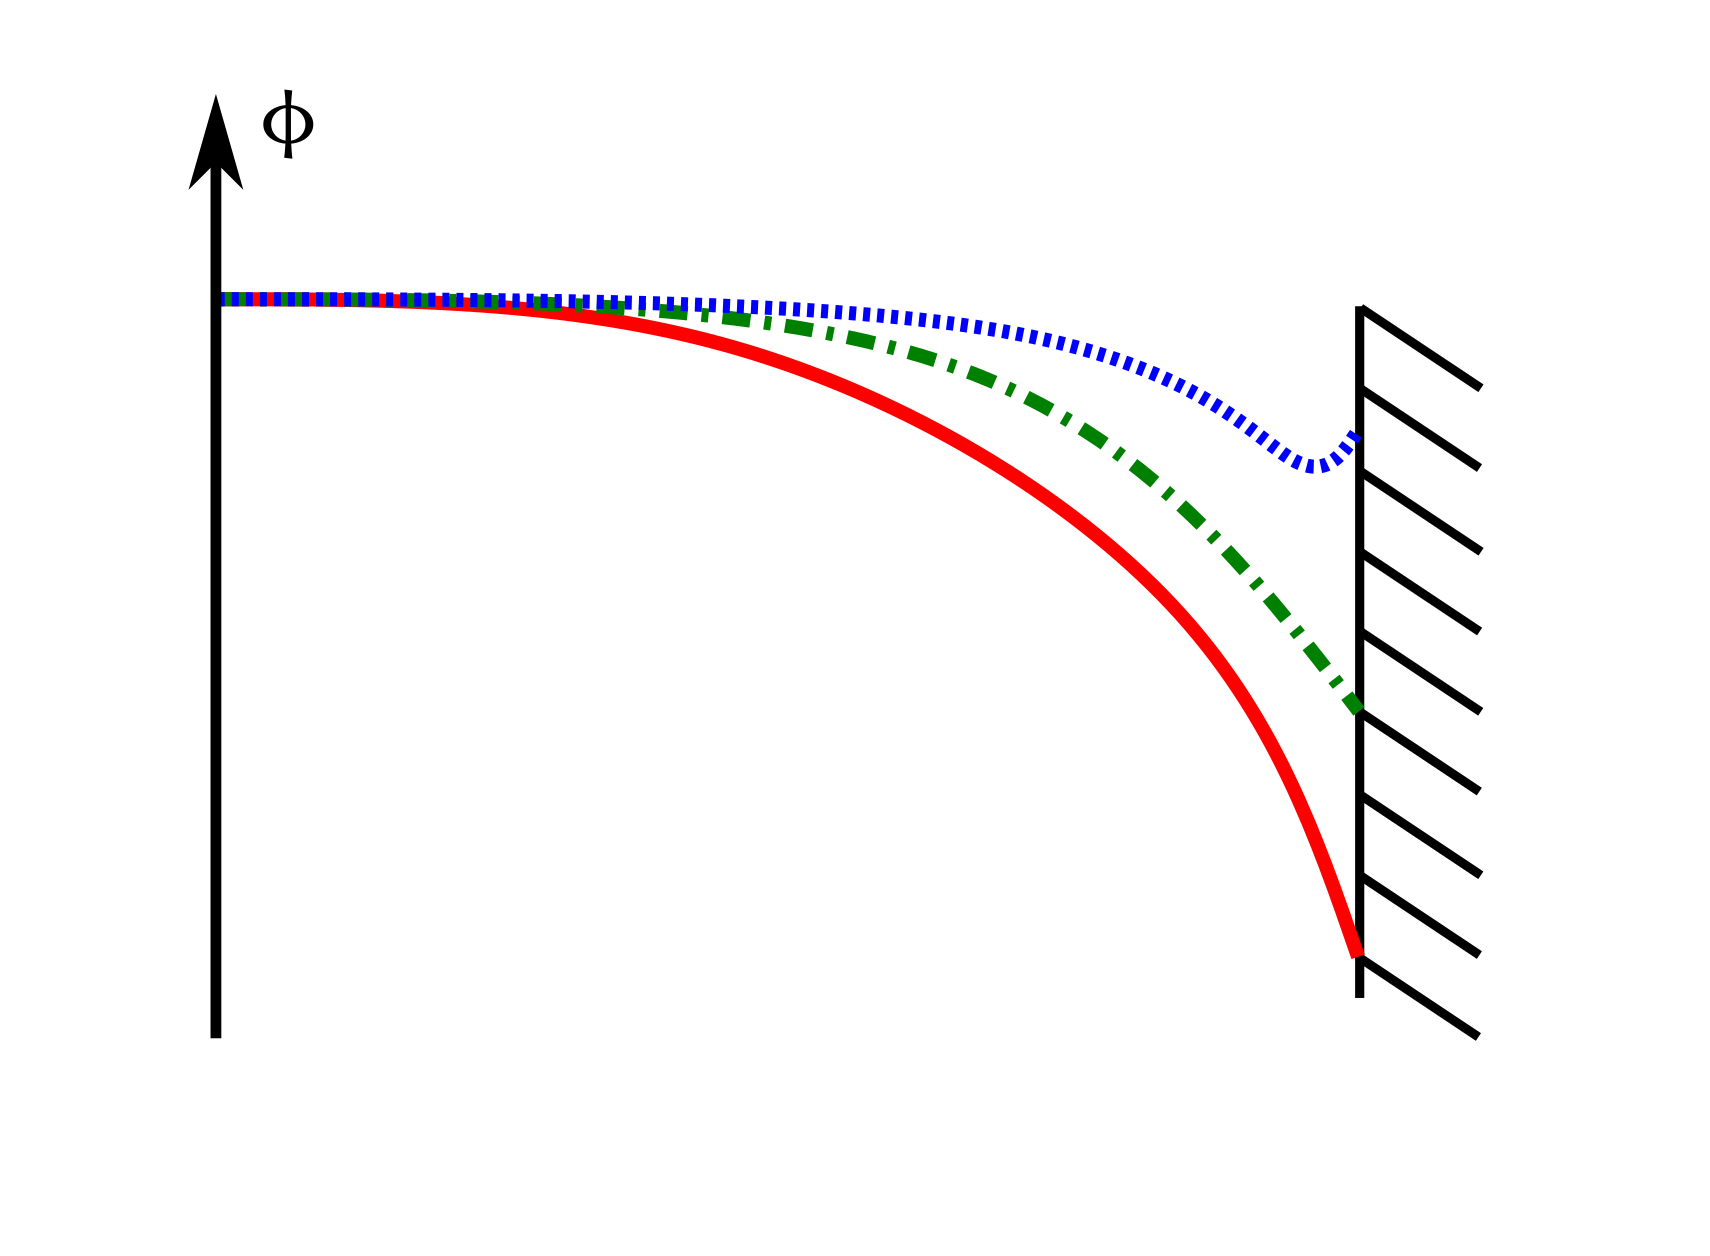
\includegraphics[width=\defaultwidth]{sheath_solutions.png}
  \caption{Schematic representation of the plasma potential profile in the sheath to the wall for the three solutions coexisting solutions. The red solid line is the standard solution, with the lowest \acs{SEE} rate; the dashed blue line corresponds to the \acs{SCL} regime, with $\rate=\ratecr$; the dash-dotted green line is the intermediate solution, with an intermediate \acs{SEE} rate.  }
  \label{fig-schematic-solutions}
\end{figure}



\Cref{fig-iso_poly} shows the evolution of the sheath potential drop and the \ac{SEE} rate as a function of $\Teb$ for the case $\crover=50\,\volt$.
Both the isothermal sheath and the polytropic model using $\gamma=1.36$ are showed. 
The result of the isothermal sheath model was previously shown in \cref{fig-dphivsTe}  in \cref{ch-2}.
The branches corresponding to the three solutions S1, S2, and S3 are labeled.
The light green area highlights the temperature range with three solutions.
The lower bounds of the area is noted $\Te^2$ and the upper bound is noted $\Te^1$
\begin{figure}[!hbt]
  \centering
  \begin{tabular}{@{} cc}
    \subfigure{Iso_vs_poly_dphibis}{a}{25,18} &
    \subfigure{Iso_vs_poly_rate}{b}{20,18} 
  \end{tabular}
  \caption{Evolution as a function of the electron temperature $\Te$ for $\crover=50\,\volt$ of ({\bf a}) the plasma potential drop to the wall $\dphi$, and ({\bf b}) the SEE rate $\ratemaxw$ using the polytropic sheath model ($\gamma = 1.36$) and the isothermal sheath model. The labels S1, S2 and SCL regime correspond to the three solutions illustrated in \cref{fig-schematic-solutions}. The light green area highlights the temperature range with three solutions.}
  \label{fig-iso_poly}
\end{figure}

We see in \cref{fig-iso_poly}.{\bf a} that $\dphi$ is significantly impacted by the polytropic law.
In particular the maximum potential drop which is more than twice as high as the isothermal maximum.
In addition, we see in \cref{fig-iso_poly}.{\bf b} that the polytropic sheath model predicts a \ac{SEE} rate smaller than the isothermal model.


\subsection{Theoretical values of the critical electron temperatures} \label{subsec-theo_Tecr}

As shown in \cref{fig-costfunction}, for a given $\Te$ the \ac{LHS} of  \cref{eq-costseepoly} presents a local minimum and a local maximum, labeled A and B respectively.
Therefore, there exist two values of $\Te$ for which either the minimum or the maximum of the \ac{LHS} crosses exactly the horizontal axis.
These values, noted $\Te^1$ and $\Te^2$ corresponds to upper and lower bounds of the electron temperature range over which the three solutions, respectively.
These threshold temperatures can be seen for $\gamma=1.36$ in \cref{fig-iso_poly}, where $\Te^1\simeq 55\,\volt$ and $\Te^2\simeq 35\,\volt$ 

\paragraph{Maximum electron temperature value for regime {\bf III}, $\Te^1$\\}

The first critical electron temperature  $\Te^1$  corresponds to the maximum temperature of the root S1, which is the usual monotonic sheath (corresponding to regime {\bf III}).
It is defined as the temperature for which the the local maximum B crosses the line $f(\chi)=0$.
As it is a double solution, it corresponds to the solution of \cref{eq-costseepoly} that is also a solution of its derivative with respect to $\chi$.
Once again, the equation is not trivial, and cannot be solved analytically, thus we solve it numerically.

\begin{figure}[hbt]
  \centering
  \begin{tabular}{@{} cc}
    \subfigure{Maximum_Te1_epsilon.pdf}{a}{20,20} &
    \subfigure{Maximum_Te1_gamma.pdf}{b}{20,15} \\
  \end{tabular}
  \caption{Variation of $\Te^1$  ({\bf a})  as a function of $\crover$ for two values of $\gamma$, and ({\bf b})  as a function of $\gamma$ for two values of $\crover$.}
  \label{fig-Te1_epsi}
\end{figure}

\Cref{fig-Te1_epsi} shows the variation of $\Te^1$ as a function of   $\crover$  and $\gamma$.
We see that the maximum temperature $\Te^1$ increases linearly with $\crover$.
This was expected, as in \cref{eq-costseepoly}, the only time that $\Teb$ is explicitly present is in the term $\frac{\Teb}{\crover}$.
On the other hand, the variation with $\gamma$ follows a power law, monotonically increasing.

\paragraph{Minimum electron temperature value for regime {\bf I}, $\Te^2$\\}

The minimum electron temperature value for regime {\bf I}, $\Te^2$, corresponds to the case where the electron temperature at the wall induces exactly an emission rate $\ratemaxw (\Tew) = \ratecr$.
Noting $C_1 = \frac{\ratecr - \sigo}{1-\sigo} = 0.964$, we obtain
\begin{equation} \label{eq-Te2}
  (1-\ratecr) \lp 2 - \frac{C_1 \crover}{2 \Te^2} \rp^{\frac{1}{(\gamma-1)}} \sqrt{\frac{C_1 \crover}{2 \Te^2}} = \sqrt{\frac{4 \gamma \pi m_e}{m_i}}
\end{equation}

\Cref{eq-Te2} is solved numerically.
The solutions for different values of $\crover$ and $\gamma$ are shown in \cref{fig-Te2_epsi}.
As for $\Te^1$, $\Te^2$ increases linearly with $\crover$, and also increases slowly with $\gamma$


\begin{figure}[hbt]
  \centering
  \begin{tabular}{@{} cc}
    \subfigure{Maximum_Te2_epsilon.pdf}{a}{20,25} &
    \subfigure{Maximum_Te2_gamma.pdf}{b}{20,20} \\
  \end{tabular}
  \caption{Variation of $\Te^2$  ({\bf a}) as a function of $\crover$ for two values of $\gamma$, and ({\bf b}) as a function of $\gamma$ for two values of $\crover$.}
  \label{fig-Te2_epsi}
\end{figure}


\subsection{Resolution of the sheath equation} \label{subsec-sol_sheat_see}
\inlinenote{should I keep this section ?}

\Cref{fig-rso_crit_see} shows the evolution of the sheath potential drop with the electron temperature for different values of $\crover$.
It is similar to \cref{fig-dphivsTe} but with the use of a polytropic state law for the electrons.
Two main aspects differ compared to the isothermal model\string: the multiple solutions and the maximal electron temperature of the first solution.

\begin{figure}[hbt]
  \centering
  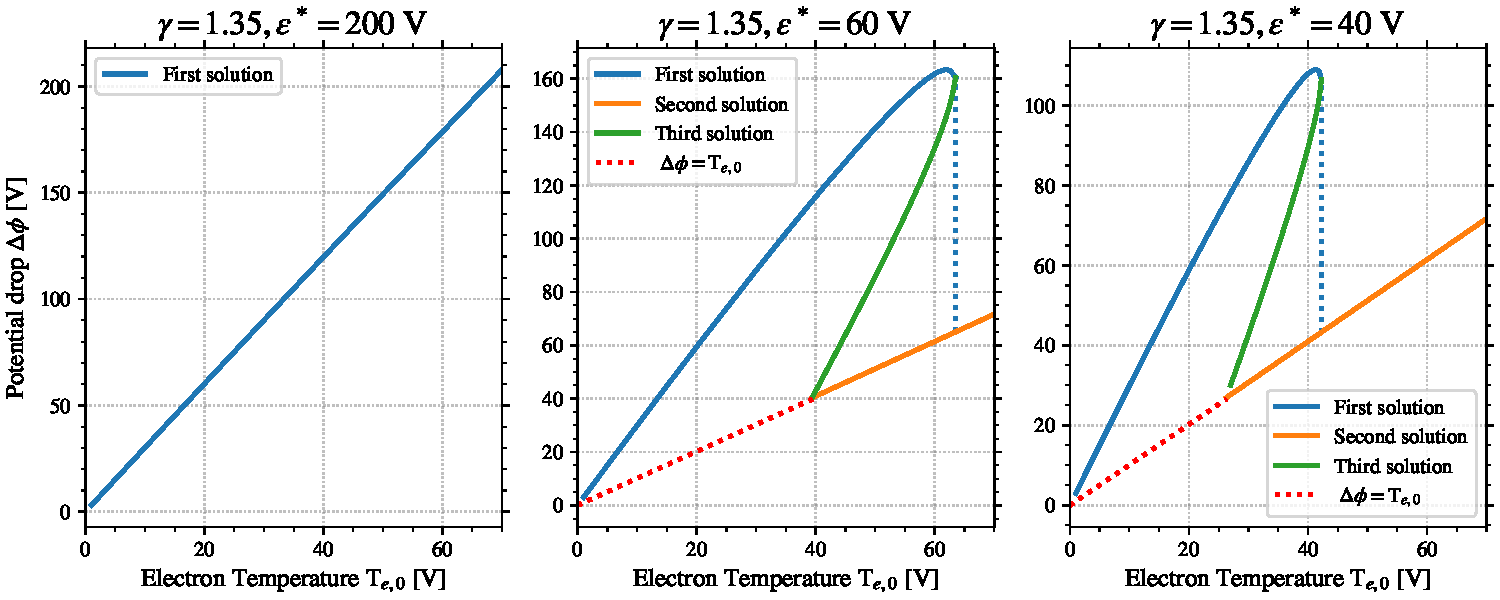
\includegraphics[width=\textwidth]{Potential_drop_poly_see.pdf}
  \caption{ Plasma potential drop to the wall as a function of the electron temperature for different values of the cross-over energy $\crover$ using \cref{eq-costseepoly}. It is the same results as  \cref{fig-dphivsTe} but with polytropic electron of index $\gamma=1.35$.}
  \label{fig-rso_crit_see}
\end{figure}

We observe in \cref{fig-rso_crit_see} that the electron temperature in the center $\Teb$ can be much higher before the inversion of the plasma sheath potential, compared to \cref{fig-dphivsTe}.
Indeed, the polytropic state law reduces the electron temperature at the wall, hence decreases the electron emission rate for a given $\Teb$.
Consequently, the electron bulk temperature can access higher temperature, compared to the one observed in \cref{fig-dphivsTe}.
Moreover, we see that the critical temperature for $\crover=40 \,\volt$ is close to $\Te=40\,\volt$, which is consistent with the transition between the regimes {\bf III} and {\bf II} observed in the \ac{PIC} simulations.

In addition, for some values of electron temperature, there are three solutions.
This could explain the oscillations observed in regime {\bf II}.
Indeed, when the electron temperature increases, the sheath follows the first solutions.
When the critical electron temperature is reached, the sheath jumps to the third solution.
It corresponds to the \ac{SCL} regime with an inverted sheath.
There, the electron temperature in the bulk decreases because of the increased electron power losses at the wall.
The electron temperature decreases until the second critical temperature, which corresponds to the moment when the third solution disappear, so that the sheath jumps back to the first solution.
We do not expect the third solution in-between to be observed in the simulations.

Obviously, the current model supposes that the polytropic index is constant.
However, we saw in the \ac{PIC} simulations that it increases from $\gamma = 1.34$ to $1.59$.
Hence, the exact values of the critical temperature may not exactly correspond to the one observed in the simulations.
On the other hand, we can expect the overall behavior not to be significantly affected.

\vspace{1em}
To summarize, the polytropic law is combined with electron emission to model the sheath.
The model obtained is richer than the usual isothermal model, as it allows multiple values of potential drop to the wall for the same electron bulk temperature.
This model only uses the electron bulk temperature and self-consistently computes both the potential drop and the electron emission rate.
It is compared in the next section to the \ac{PIC} simulation results.


\let\rightmark=\oldrightmark
